%% Local variables:
% TeX-file: main
%% End:

\title{Polimorfismo e Acoplamento Dinâmico}

\frame{\maketitle}

\begin{frame}{Polimorfismo}

  Substituição ou redefinição de atributos e métodos da superclasse
  para adequação às características da subclasse.  

Métodos: 
\begin{description}
\item[Sobrecarga] ({\it overload})-- fornecer mais de um método com o
  mesmo nome, mas com diferentes assinaturas para distinguí-los;

\item[Sobrescrita] ({\it overriding}) -- substitui a implementação
  daquele método com a sua própria. As assinaturas podem ser
  idênticas, mas o tipo de retorno pode variar de maneira particular.

\end{description}

\end{frame}

\begin{frame}[fragile]{Sobrecarga}{Redefinição}
  \footnotesize

  O acomplamento do método é feito de acordo com a sua \alert{assinatura}.

\begin{center}
  \begin{tikzpicture}
  \begin{class}[]{Triangulo}{0,0}
      \operation{desenhar()}
      \operation{desenhar(ct : TipoTriangulo)}
      \operation{apagar()}
    \end{class}
  \end{tikzpicture}
\end{center}

 \begin{lstlisting}[]
class Triangulo {
      enum TipoTriangulo{isosceles, retangulo}; 

      void desenhar() { 
        System.out.println("Triangulo.desenhar()");
      }
      void desenhar(TipoTriangulo ct) {
      	   System.out.println(ct);
      }
      void apagar() { 
      	   System.out.println("Triangulo.apagar()");
      }   }
  \end{lstlisting}

\end{frame}

\begin{frame}{Sobrescrita}{\it Overrinding}

\begin{tikzpicture}
  \begin{class}{Forma}{1,0}
	\operation{desenhar()}
	\operation{apagar()}
  \end{class}

  \begin{class}[text width=2.5cm]{Retangulo}{-4.5,-3.5}
	\inherit{Forma}
	\operation{desenhar()}
	\operation{apagar()}
  \end{class}

 \begin{class}[text width=2.5cm]{Circulo}{-1,-3.5}
 	\inherit{Forma}
	\operation{desenhar()}
	\operation{apagar()}
  \end{class}

  \begin{class}[text width=2.5cm]{Triangulo}{3,-3}
  	\inherit{Forma}
	\operation{desenhar()}
	\operation{apagar()}
  \end{class}
\end{tikzpicture}
\end{frame}

\begin{frame}[fragile]{Sobrecarga}{Exemplo}

\begin{center}

\begin{lstlisting}

class Forma {
      void desenhar() { }
      void apagar() { }
}

class Circulo extends Forma {
      void desenhar() { 
            System.out.println("Circulo.desenhar()");
      }
      void apagar() { 
            System.out.println("Circulo.apagar()");
      }
}
\end{lstlisting}

\end{center}

\end{frame}

\begin{frame}[fragile]{Sobrecarga}{Exemplo}

\begin{center}

\begin{lstlisting}

class Forma {
      void desenhar() { }
      void apagar() { }
}

class Quadrado extends Forma {
      void desenhar() { 
            System.out.println("Quadrado.desenhar()");
      }
      void apagar() { 
            System.out.println("Quadrado.apagar()");
      }
}
\end{lstlisting}

\end{center}

\end{frame}

\begin{frame}[fragile]{Sobrecarga}{Exemplo}

\begin{center}

\begin{lstlisting}
class Forma {
      void desenhar() { }
      void apagar() { }
}

class Triangulo extends Forma {
      void desenhar() { 
            System.out.println("Triangulo.desenhar()");
      }
      void apagar() { 
            System.out.println("Triangulo.apagar()");
      }
}
\end{lstlisting}

\end{center}

\end{frame}

\begin{frame}[fragile]{Acoplamento Dinâmico}{\it Dynamic binding}

  \footnotesize No acoplamento dinâmico ({\it dynamic binding}), o
  método a ser executado é vinculado à referência ao objeto durante a
  execução do código de acordo com o tipo do objeto no momento da
  execução.

\begin{lstlisting}
public class PoliMain {
      public static Forma sortearForma () {
            switch( (int)(Math.random() * 3) ) {
                  default:
                        case 0: return new Circulo();
                        case 1: return new Retangulo();
                        case 2: return new Triangulo();
                  }
            }
      public static void main(String[] args) {
            Forma[] fs = new Forma[9];
		
            for(int i=0; i< fs.length; i++)
                  fs[i] = sortearForma( );

            for(int i=0; i<fs.length; i++)
                  fs[i].desenhar();
            }}
\end{lstlisting}

\end{frame}

\begin{frame}{Acoplamento dinâmico}{Visualização}
\footnotesize

\begin{tikzpicture}[bind/.style={->,>=latex,draw},
baseclass/.style={draw},
circleclass/.style={baseclass,fill=yellow},
triangleclass/.style={baseclass,fill=blue!20},
rectangleclass/.style={baseclass,fill=green!20}]

\node at (5,2) {sorteio:\bf \only<1>{0} \only<2>{2} \only<3>{1}\only<4>{2}};

\foreach \y in {0,1,...,8}{
	 \node[rectangle,draw] (ref\y) at (-2,-.465*\y) {Forma\@@ref\y};
}

\path<1->[bind] (ref0.east) ->  (3,2) node[circleclass] {Circulo};
\path<2->[bind] (ref1.east) ->  (3,1) node[triangleclass] {Triangulo};
\path<3->[bind] (ref2.east) ->  (3,0) node[rectangleclass] {Retangulo};

\path<4->[bind] (ref3.east) ->  (3,-1) node[triangleclass] {Triangulo};
\path<4->[bind] (ref4.east) ->  (3,-2) node[triangleclass] {Triangulo};
\path<4->[bind] (ref5.east) ->  (3,-3) node[circleclass] {Circulo};
\path<4->[bind] (ref6.east) ->  (3,-3.75) node[rectangleclass] {Retangulo};
\path<4->[bind] (ref7.east) ->  (3,-4.5) node[circleclass] {Circulo};
\path<4->[bind] (ref8.east) ->  (3,-5.5) node[triangleclass] {Triangulo};

\end{tikzpicture}

\end{frame}

\begin{frame}[fragile]{Coerção}{\it Cast}
\footnotesize
\alert{Coerção} é a tentativa de modificar o tipo do objeto de acordo com
comportamento requerido durante a execução.
\scriptsize
\begin{lstlisting}
class Triangulo extends Forma {
      void desenhar() { 
            System.out.println("Triangulo.desenhar()"); }
      void apagar() { 
            System.out.println("Triangulo.apagar()"); }
      void somarAngulos() {
      System.out.println(“Soma angulos internos=180”); }
}
public class CoercaoMain {
      public static void main(String[ ] args) {
            Forma[ ] fs = { new Forma(),
                            new Triangulo() };
		
            fs[0].desenhar();
            fs[1].apagar();
             /* mas fs[0] não é triangulo?!!! */	
            ( (Triangulo) fs[1] ).somarAngulos();
            ( (Triangulo) fs[0] ).somarAngulos();
      } }
\end{lstlisting}

\end{frame}

\begin{frame}{Coerção}{Visualização}

\begin{tikzpicture}

\foreach \y in {0,1}{
	 \node[fill=gray!20,rectangle,draw] (ref\y) at (-2,-.465*\y) {Forma\@@ref\y};
}

 \begin{class}[text width=2.5cm,fill=gray!20]{Forma}{2,1}
	\operation{desenhar()}
	\operation{apagar()}
  \end{class}


 \begin{class}[text width=2.5cm,fill=blue!20]{Triangulo}{2,-2}
	\operation{desenhar()}
	\operation{apagar()}
	\operation{somarAngulos()}
  \end{class}

\path[->, draw] (ref0.east) -- (.6,.5) node{};
\path[->, draw] (ref1.east) -- (.6,-2.5) node{};


\draw<2>[line width=1mm, red] (0,1) -- (4,-1.5);
\draw<2>[line width=1mm, red] (4,1.5) node[above] {Não é {\tt Triangulo}} -- (0,-1);

\end{tikzpicture}

\end{frame}

\begin{frame}[fragile]{Coerção Segura}{\tt instanceof}

\begin{lstlisting}
public class CoercaoSeguraMain {
    public static void main(String[] args) {
        Forma[ ] fs = { new Forma(), new Triangulo() };
		
            fs[0].desenhar();
            fs[1].apagar();
                
            if( fs[1] instanceof Triangulo )
                ( (Triangulo) fs[1] ).somarAngulos();

            if( fs[0] instanceof Triangulo )
            ( (Triangulo) fs[0] ).somarAngulos();
    }
}
\end{lstlisting}

\end{frame}

\begin{frame}{Polimorfismo e Acoplamento Dinâmico}{Conclusões}

  \begin{itemize}
  \item  Vantagens
    \begin{itemize}
      \item Flexibilidade;
      \item Incorporação das técnicas de ``herança'' à linguagem.
    \end{itemize}

  \item Desvantagens
    \begin{itemize}
    \item Perda de performance devido ao uso da memória heap;
    \item Aumenta a necessidade de checagem de condições de erro durante a
      execução que eram verificadas em tempo de compilação por
      compiladores de linguagens estáticas.
    \end{itemize}
  \end{itemize}

\end{frame}

\begin{frame}[fragile]{Referências}

\begin{thebibliography}{Arnold, 2007}

 \bibitem[Eckel, 1998]{eckel1998}
 		    Bruce Eckel.
 \newblock 	   {\em Thinking in Java}.
\newblock	   Prentice-Hall, 1998.

\bibitem[Arnold, 2007]{arnold2007}
  Ken Arnold, James Gosling, David Holmes.
\newblock  {\em A Linguagem de Programação Java}.
\newblock 4$^a$ edição, Bookman, 2007, 
\end{thebibliography}

\end{frame}
